\documentclass{beamer}
% \usetheme[]{Frankfurt}
\usepackage{tikz}
\usepackage{physics}
\usetikzlibrary{shapes,arrows}
\usepackage{handbook}
\usepackage{media9}
\usepackage{multicol}
\usepackage[sorting=none]{biblatex}

\addbibresource{handbook.bib}
\begin{document}
\title{Praxis II Handbook}   
\author{QiLin Xue}
\date{\today} 
\hbadness=99999 % we're bad students
\hfuzz=100pt % wide bois begone

\frame{\titlepage} 

\frame{\frametitle{Table of Contents}
\begin{multicols}{2}
    \tableofcontents
\end{multicols}
} 


\section{Introduction} 
\frame[allowframebreaks]{\frametitle{Introduction}
    This handbook is intended to serve as a reference for engineering design, drawing upon the experience of the author, QiLin Xue, during his first year as an Engineering Science student as UofT.
    \begin{enumerate}
        \item I will go over my positionality as an engineering student and my personal engineering design process.
        \item I will then focus on the specific tools, models, and frameworks I used for each part of my design process
        \item I will supplement the above with evidence from \textit{nine} engineering projects, as well as what I learned from each.
    \end{enumerate}
    \newpage
    \textbf{Why is this in slides?} The purpose of this handbook is supposed to be for \textit{future} reference for myself and other people. Having it as slides has two advantages:
    \begin{itemize}
        \item It forces me to be concise, and there's only so much I can fit in one slide. No one wants to spend their time reading irrelevant text.
        \item As it will be discussed in my positionality, I take a great interest in education, and having it in slides will potentially make this a great teaching tool in the future as well.
    \end{itemize}
    I hope you are able to learn about how I approach engineering design in this handbook.
}

\section{Positionality} 
\frame[allowframebreaks]{\frametitle{Positionality}
I identify myself as both an \textbf{engineering student} and an \textbf{educator}:
\begin{itemize}
    \item As an \textit{engineering student}, I enjoy learning new things, both in class, and outside. Some recent topics I am learning include microcontrollers, aerodynamics, and quantum mechanics.
    \item As an \textit{educator}, I enjoy exposing other people to math and physics. I work as a teaching assistant at \textit{AoPS}, which teaches contest math and physics, as well as doing research in physics education.
\end{itemize}
I therefore approach engineering problems and the design process from these two different perspectives. However, it is also important to recognize the biases that affect this handbook:
\begin{itemize}
    \item As a student, I am still new to formal engineering design. As a result, I may not have a full understanding of the various tools, models, and frameworks described in this handbook simply because of the limited sample size.
    \item Another bias as a student that affects this handbook is that the main purpose is to get marks for the Praxis II course. I hope this doesn't greatly affect this handbook, but it feels important to disclose that this is a required part of my coursework for any future readers.
\end{itemize}
and the biases that approach my engineering design work:
\begin{itemize}
    \item This will be elaborated on further, but one of my biggest values involve taking a lot of high risk opportunities. The philosophy behind it is that failing as a student does not have life changing consequences. As a result, I will often try to find esoteric solutions and may gloss over simple ones.
\end{itemize}
}

\section{Values} 
\frame[allowframebreaks]{\frametitle{Values}
I have three main values:
\begin{itemize}
    \item \textbf{Ambition:} I like taking risks and doing difficult tasks, even if it means I might fail. This comes from my position as a student: I'm here to first and foremost learn and I personally learn more through failure than through success.
    \begin{itemize}
        \item This is reflected when brainstorming ideas. I am not afraid of trying to pursue difficult and challenging designs that might come with a lot of risk.
    \end{itemize}
    \item \textbf{Accountability:} If I say I'm going to complete a task by this date, I will complete the task by that date. If I cannot, I will give a heads up well in advance. This is a simple philosophy that I live by and in a team setting, I expect my teammates to do the same.
    \item \textbf{Balance:} Academics and professional life isn't everything. While I always strive to the best I could, I do not want to sacrifice my mental or physical health in order to do so.
\end{itemize}
}


\section{Engineering Design Process}
\frame[allowframebreaks]{\frametitle{Engineering Design Process}

    \tikzstyle{decision} = [rectangle, draw, fill=red!20, 
    text width=5em, text centered, rounded corners, minimum height=2em]
    
    \tikzstyle{major} = [rectangle, draw=yellow!90, thick, fill=yellow!20, 
    text width=5.5em, text centered, rounded corners, minimum height=2em]
    \tikzstyle{sub} = [rectangle, fill=red!20, 
    text width=5em, text centered, rounded corners, minimum height=2em]

    \tikzstyle{block} = [rectangle, draw, fill=blue!20, 
    text width=5.5em, text centered, minimum height=2em]
    \tikzstyle{line} = [draw, -latex', thick]
    \tikzstyle{O} = [draw, -latex', thick]

    \begin{center}
        \begin{tikzpicture}[node distance = 3cm, auto, scale=0.5]
            
            % STAKEHOLDERS
            \node [major] (Framing) {Framing};
            \node [major, right of = Framing] (Diverging) {Diverging};
            \node [major, right of = Diverging] (Converging) {Converging};
            \node [major, right of = Converging] (Representing) {Representing};

            \node [block, below of = Framing, node distance = 1.2cm, xshift=0.9cm, text width=10em] (Requirements) {\small Develop \\ Requirements Model};

            \node [block, right of = Requirements, node distance = 3cm, yshift=-1.2cm, text width=10em] (Iteration) {\small Perform \\ Iterative Design};

            \node [block, right of = Iteration, node distance = 3cm, yshift=-1.2cm, text width=8em] (Testing) {\small Execute \\ Rigorous Tests};

            \node [block, right of = Testing, node distance = 2.2cm, yshift=-1.2cm, text width=6em] (Present) {\small Present to \\ Other People};

            \node [sub, below of = Requirements, node distance = 5cm, xshift=-3em] (Bias) {Identify Bias}; 
            \node [sub, right of = Bias, node distance = 2.7cm] (Research) {Research Informed}; 
            \node [sub, right of = Research, node distance = 2.7cm] (Tools) {Brainstorm Ideas}; 
            \node [sub, right of = Tools, node distance = 2.7cm] (Prototype) {Proto typing}; 

            \path [line, blue] (Requirements) |- (Iteration);
            \path [line, blue] (Iteration) |- (Testing);
            \path [line, blue] (Testing) |- (Present);

            \path [line, red] (Iteration) |- (Requirements);
            \path [line, red] (Testing) |- (Iteration);
            \path [line, red] (Present) |- (Testing);

            \path [line, dotted] (Bias) -- (Requirements);
            \path [line, dotted] (Research) -- (Requirements);

            \path [line, dotted] (Bias) --       (Iteration);
            \path [line, dotted] (Research) --   (Iteration);
            \path [line, dotted] (Tools) --      (Iteration);
            \path [line, dotted] (Prototype) --  (Iteration);

            \path [line, dotted] (Bias) --       (Testing);
            \path [line, dotted] (Research) --   (Testing);
            \path [line, dotted] (Prototype) --  (Testing);

            \path [line, dotted] (Research) --   (Present);
            \path [line, dotted] (Prototype) --  (Present);
        \end{tikzpicture}
    \end{center}
    \newpage
    This is a high level overview of my engineering design process. Everything I do can be loosely categorized using the modified \textbf{FDCR} process:
    \begin{itemize}
        \item \textbf{Framing:} What are the requirements? How can we conduct quality research?
        \item \textbf{Diverging:} What are some effective ways to brainstorm ideas? 
        \item \textbf{Converging:} How can we build prototypes, test, narrow down our set of ideas, and re-diverge?
        \item \textbf{Representing:} How can we present our ideas to other people in an effective manner?
    \end{itemize}
    In the above flowchart, note that I frequently move back and forth between the stages. 
    \vspace{2mm}

    The red boxes at the bottom represent the main engineering themes that will be present throughout each part of the process.
    \newpage
    I approach each stage from a different position:
    \begin{itemize}
        \item When developing a \textbf{requirements model}, I approach it from the position of an educator. One of the most important things in teaching is recognizing and addressing hidden assumptions, and that is exactly what I ask myself here:
        \begin{itemize}
            \item What assumptions am I making? When are they valid? How can I rigorously justify them?
        \end{itemize}
        This is often the most difficult part of physics problems, and also the hardest part about design. Being able to recognize my own biases and ensuring everything in the framing process is well justified is hard, but critical for success.
        \item When I perform \textbf{iterative design} and performing \textbf{rigorous tests}, I do some from the perspective of an engineering student. What tools can I use to get more designs? How should I compare these two designs? I am still learning, so I try to use a variety of new tools for each project.
        \item When \textbf{presenting} to other people, I again approach this from the perspective of an educator. I ask myself:
        \begin{itemize}
            \item How would I present the design to a young student? What about someone my age? What about an industry leader?
        \end{itemize}
        This sort of questioning allows me to holistically evaluate how confident I am that the design meets the requirements.
        \begin{example}
            After I was done the first stage of my aerodynamics project at UofT's \textbf{rocketry team}, I wanted to ensure I could defend my design. I gave a presentation to two groups: one to other people working in the aerodynamics subdivision of the team, and one at a general meeting. Being able to present the design to people who may not be familiar with aerodynamics forced me to make sure I wasn’t hiding behind jargon and presenting it to very knowledgeable people gave me valuable feedback that I am currently taking and improving on the design.
        \end{example}
    \end{itemize}
}

\section{Overview of Projects}
\frame[allowframebreaks]{\frametitle{Overview of Projects}
Throughout this handbook, I will be making references to the following projects which I started in the 2020-2021 school year. As part of the Praxis I/II course:
\begin{itemize}
    \item \textbf{Design Brief:} My team wrote a design brief highlighting the opportunity to reduce the negative physiological impacts associated with Computer Vision Syndrome for students at UofT.
    \item \textbf{Diverging Sprint:} My team provided a detailed description of various ideas that would solve the opportunity of making mental health friendly plant containers.
    \item \textbf{Alpha Release:} My team developed a prototype mouse to alleviate the pain Carpal Tunnel Syndrome patients may feel when using a computer.
    \item \textbf{Showcase:} The culmination of Praxis II, my team developed a tool to assist Parkinson's patients in rose grafting. 
\end{itemize}
\newpage
Outside the course:
\begin{itemize}
    \item \textbf{UTAT:} Developed nose cone and fin optimization code for the University's rocketry team.
    \item \textbf{Civ Bridge:} Designed and optimized two bridges to complete a challenge set in the CIV102 course.
    \item \textbf{Gomoku Tournament:} Created a mini-max AI to compete in a gomoku tournament.
    \item \textbf{UTAG:} An ongoing student-led project where we are creating automatic sustainable plant boxes.
\end{itemize}
}
\section{Framing}
\frame[allowframebreaks]{\frametitle{Framing}
\textit{Motivation:} Framing is vital in building a solid foundation for engineering design. When presented with an opportunity, different people have various assumptions about what the design \textit{should} or shouldn't do. In this stage, it is important to understand the \textbf{stakeholders}, the \textbf{requirements}, and the \textbf{existing solutions}. The following tools assist in this process:
\begin{itemize}
    \item Requirements Model
    \item Flowchart Visualization
    \item Research Tools
\end{itemize}
}

\subsection{Requirements Model}
\frame[allowframebreaks]{\frametitle{Requirements Model}
    A requirements model contains of the following elements:
    \begin{itemize}
        \item \textbf{Stakeholders:} Who are the stakeholders, and what are their values?
        \item \textbf{Objectives:} What should the design should?
        \begin{itemize}
            \item High level: Very broad and general, supposed to encapsulate the big ideas.
            \item Low level: Very specific, supposed to make you think about specific design choices.
        \end{itemize}
        \item \textbf{Metrics:} A quantifiable measurement that can be made for every design. Can be in a a rubric style.
        \item \textbf{Criteria:} What is preferred for each metric.
        \item \textbf{Constraints:} What must be satisfied for each metric.
    \end{itemize} 

    \newpage
    \begin{example}
        The following is an example of the requirements surrounding a detailed objective from our Praxis II RFP. Notice that the low level objective is tied to a high level objective.
        \begin{center}
            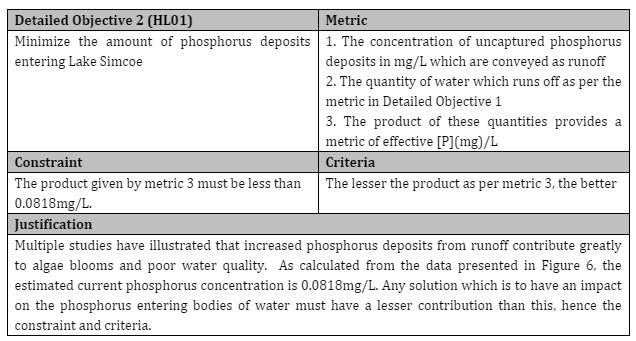
\includegraphics[width=0.8\linewidth]{handbook/objective_example.jpg}
        \end{center}
    \end{example}
    
    \newpage
    \begin{example}
        \begin{columns}
            \begin{column}{0.4\textwidth}
                Additionally, as part as our framing process for UTAG, we have separate framing sections for each subteam. The following revolves around the requirements of the lighting system, which was performed by my colleagues, not me.
            \end{column}
            \begin{column}{0.6\textwidth}
                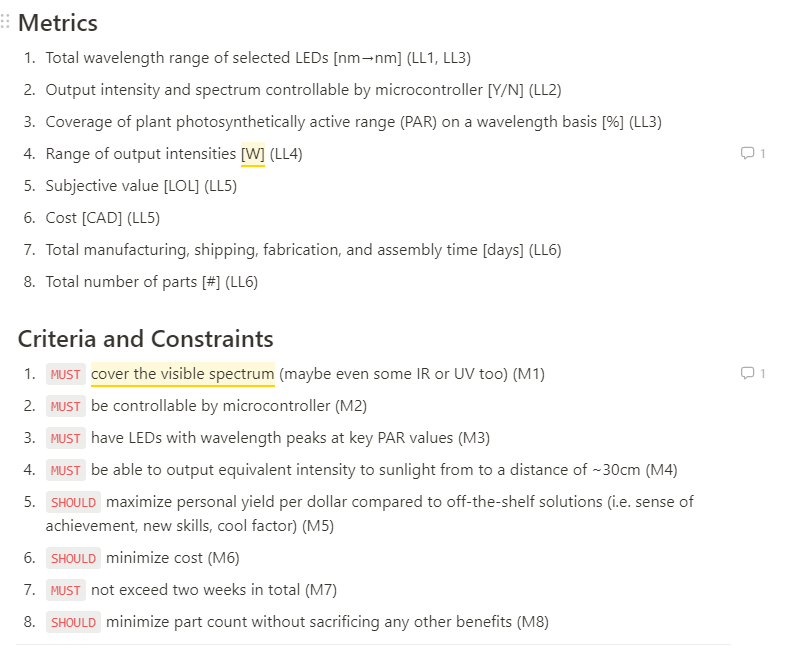
\includegraphics[width=\linewidth]{handbook/notion.png}
            \end{column}
        \end{columns}
    \end{example}
}
    
    \subsubsection{Flowchart Visualization}
    \frame[allowframebreaks]{\frametitle{Flowchart Visualization}
    \begin{center}
    \begin{columns}
        \begin{column}{0.4\textwidth}
            \textit{Motivation:} For complex projects, one may have several stakeholders who may not have the same requirements. To help visualize it, drawing a flowchart of the requirements may be a good idea:
            \vspace{2mm}

            The image to the right is an example of a flowchart from my Praxis II RFP. 
        \end{column}
        \begin{column}{0.6\textwidth}
            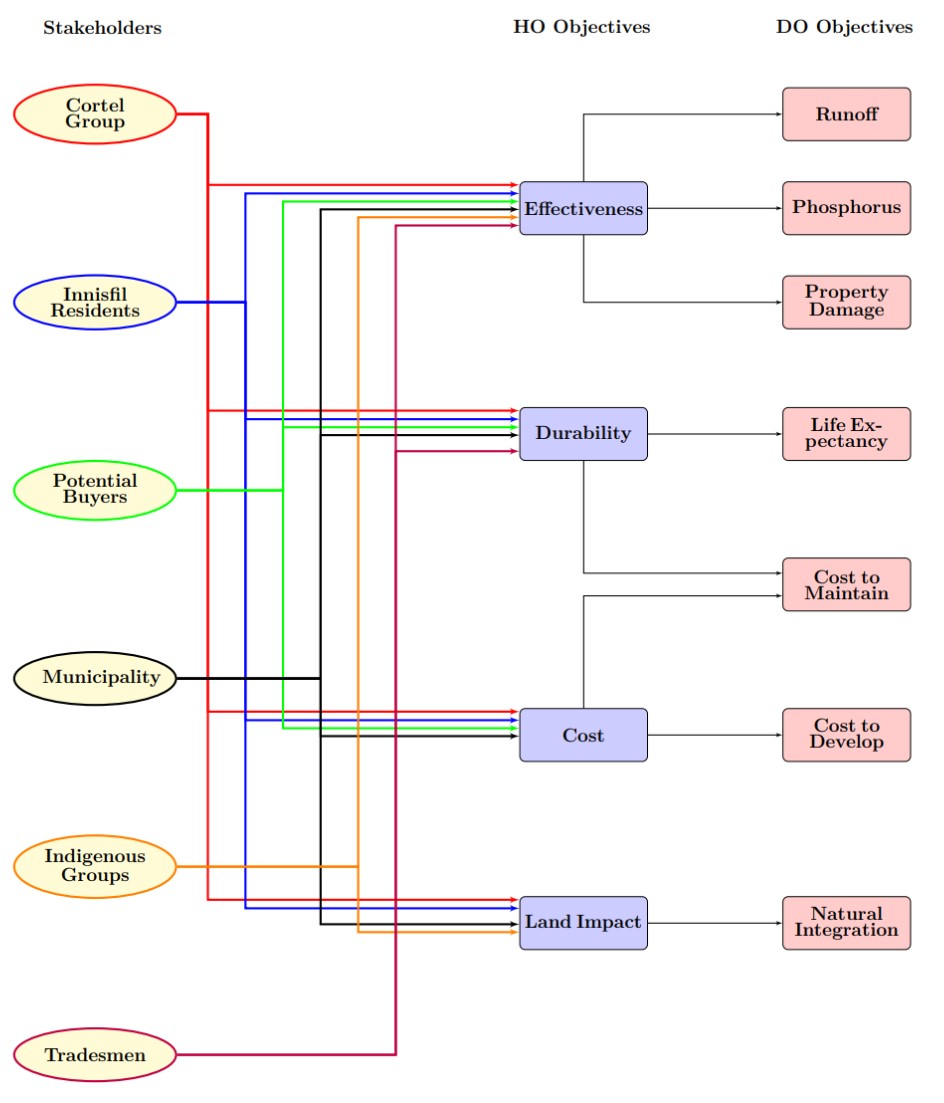
\includegraphics[width=\linewidth]{handbook/flowchart.jpg}
        \end{column}
    \end{columns}
\end{center}
}

\subsection{Research}
\frame[allowframebreaks]{\frametitle{Research}
  While a good design requires originality, it is not a wise idea to do everything from scratch. Building off of the work other people have done (and giving credit) can assist in:
  \begin{itemize}
      \item Identifying specific needs
      \item Evaluating potential designs
      \item Inspiring new ideas
  \end{itemize}
  However, there is also a \textbf{curse of information:} with so many different sources online, it is important to be able to identify which ones are reliable.
}

\subsubsection{CRAAP Test}
\frame[allowframebreaks]{\frametitle{Research: CRAAP Test}
  The \textbf{CRAAP test} is a \textit{tool} to evaluate how reliable (or crappy) a source is. It is an acronym for\cite{craap}:
  \begin{itemize}
      \item \textbf{Currency:} When was the information published? Could there be major changes between then and now?
      \item \textbf{Relevance:} Does this source really satisfy my needs?
      \item \textbf{Authority:} Who wrote this? How can I know to trust them?
      \item \textbf{Accuracy:} How do I know the information presented is correct?
      \item \textbf{Purpose:} Why did the author write this? Do they have an agenda (either directly stated), or is it hidden?
  \end{itemize}
  \newpage 

  During our Praxis I Design Brief, we used a paper describing the management of digital eye strain, found \href{https://www.tandfonline.com/doi/full/10.1111/cxo.12798}{here}. We conducted the CRAAP test on the paper, and the results are summarized below:
  %TODO: Cite https://sci-hub.se/10.1111/cxo.12798
  \begin{itemize}
      \item \textbf{Currency:} The paper was written in 2018, before covid-19 forced students to learn from home. Thus, numbers reported may not reflect the current situation. However, we see no reason to believe the experimental results would change.
      \item \textbf{Relevance:} The paper was written from an optometry perspective, so it focused on very technical elements. As a result, it may not have covered sufficient breadth.
      \item \textbf{Authority:} The authors are fellows of the American Academy of Optometry, where additional rigorous qualifications need to be met.
      \item \textbf{Accuracy:} We cannot evaluate the accuracy based off of this one article, but using \textit{research triangulation}, we were able to verify that the information provided was accurate.
      \item \textbf{Purpose:} This paper was published in an optometry journal, so it was intended for other optometrists such that they can make better recommendations. We did not find any hidden agenda.
  \end{itemize}
  Much of the information related to credibility can be found on the first page of the paper\cite{Colesbrennan2019}:
  \begin{center}
      
\includegraphics[width=0.8\linewidth]{handbook/craap.jpg}
  \end{center}
}

\subsubsection{Triangulation}
\frame[allowframebreaks]{\frametitle{Research: Triangulation}
  \textit{Motivation:} Using only one source is dangerous, as the information can be biased. Even if the authors are trustworthy and the paper is peer reviewed, it can still have mistakes. There are three ways to perform triangulation:
  \begin{itemize}
      \item If a source has references, check that their references are reliable and that the cited information is accurately portrayed.
      \item If the source makes a claim, purposely look for other sources that make the opposing claim, if any.
      \item Collect primary evidence that either support or refute the article's claim. 
  \end{itemize}
  When writing the RFP for Praxis II, our stakeholder, a construction group, made a bold claim that the new subdivision they are building will be environmentally friendly, \textit{double} the city's population, and will enhance the experience of people already living there.
  \vspace{2mm}

  Our team thought that this was a dubious claim that was rooted in bias, as it was part of their promotional campaign. We decided to investigate the degree to which the claims were accurate via triangulation. As shown in our RFP\cite{rfp}:
  \begin{itemize}
      \item A city council meeting discussing the project, which was backed up my an environmentalist Alex Waters
      \begin{itemize}
          \item We found that Alex Waters is a ``super'' environmentalist, working as an environmental instructor for 30 years, and built his own home to be the most energy efficient in the city.
          \item There was a lot of support by current residents at the meeting. We considered the possibility that only the ones interested in the project would come, making this biased. However, we also found that a previous construction project was halted in the same room due to concerns over environmental issues. Therefore, this is likely \textit{not} the case.
      \end{itemize} 
      \item There exists a small organization that is openly against the developement of the subdivision, but emphasizes on their website that their main concern is the rapid plans, and not the idea.
  \end{itemize}
  This is just a small example of the various steps my team took during triangulation to verify claims. Additionally by doing so, we can get a \textbf{better understanding of the stakeholders} as well.
}


\section{Diverging}
\frame[allowframebreaks]{\frametitle{Diverging}
  \textit{Motivation:} Now that most\footnote{I will discuss reframing later} of the foundational work has been set, the main goal is to generate as many different ideas as possible without caring about the quality. However, this is not easy and there are several challenges:
  \begin{itemize}
      \item \textbf{Bias:} We need to prevent our own bias and assumptions from affecting the design choices.
      \item \textbf{Anchoring:} We need a wide range of creative ideas, and it is easy to revolve ideas around the initial ones.
      \item \textbf{Inclusiveness:} When working in a team setting, how can we make sure to include everyone's ideas?
  \end{itemize}
  The \textbf{tools} I will discuss in the next few slides attempt to combat these challenges.
}

\subsection{Divergence Tools}
\frame[allowframebreaks]{\frametitle{Divergence Tools}
  There are a variety of tools that can be used during the diverging process\cite{tools}. However I will only describe in detail the ones I found to be the most useful in tackling the challenges identified in the previous slide:
  \begin{itemize}
      \item Classic Brainstorming
      \item Brainwriting
      \begin{itemize}
        \item Helps with \textit{inclusiveness}
        \end{itemize}
      \item Random Input
      \begin{itemize}
        \item Helps with \textit{anchoring}
        \end{itemize}
      \item Biomimicry
      \begin{itemize}
          \item Helps with \textit{bias} and \textit{anchoring}
      \end{itemize}
  \end{itemize}
  I will also discuss the limitations of each tool and what one needs to watch out for in the future.
}

\subsubsection{Classic Brainstorming}
\frame[allowframebreaks]{
    \frametitle{Classic Brainstorming\cite{tools}}

        \textit{Motivation:} The most basic form everyone knows about and has used before. This involves writing down ideas and building upon each other freely in an open manner. This helps for projects that need to be completed quickly, such as the 24-hour hackathon I participated in. We framed the requirements for a potential project we wish to work on, and generated some ideas:

        \begin{center}
            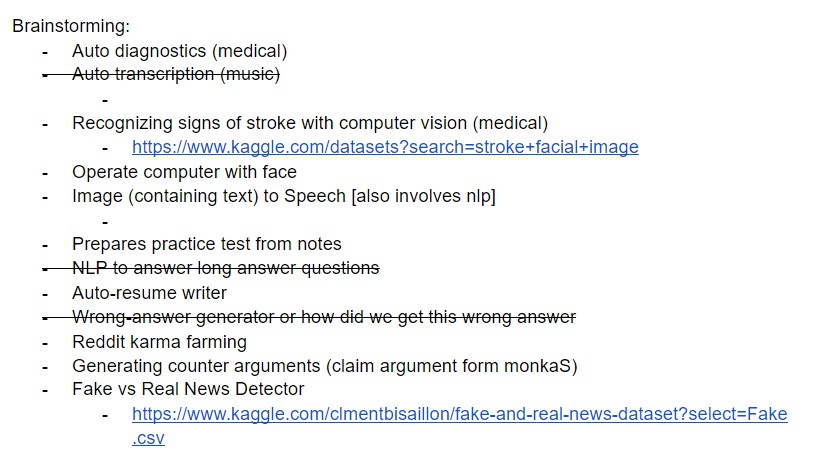
\includegraphics[width=0.8\linewidth]{handbook/classic_brainstorm.jpg}
        \end{center}

        \newpage

        The crossed out text was remnants from our converging phase. There were a lot of drawbacks, especially with \textbf{anchoring}. Looking back, we focused a lot on natural language processing (NLP) type tasks, and we didn't even consider other potential areas in artificial intelligence.
        \vspace{2mm}

        Our team also did not know each other too well, so there is a possibility that some members (who did not have a lot of ML experience) were not as comfortable sharing ideas as those who had past experience. As a result, \textbf{team dynamics} is also very important, and arguably more important than picking the right tools.
}

\subsubsection{Random Input}
\frame[allowframebreaks]{\frametitle{Random Input\cite{tools}}
    \textit{Motivation:} We wish to remove the risk of anchoring completely by having a computer generate random objects which we generate ideas off of, forcing us to be creative. Many of these ideas will be bad, but the point is to broaden the \textbf{search space}. 
    
    \begin{method}
        The idea is to move quickly and efficiently.
        \begin{enumerate}
            \item Find a random object generator like \href{https://perchance.org/object}{this}.
            \item Generate a random object and set the time for three minutes.
            \item Everyone tries to come up with ideas related to the word. Once the timer is up, move immediately.
            \item At the end, discuss ideas and new perspectives of looking at the opportunity.
        \end{enumerate}
    \end{method}
    \newpage
    \begin{example}
        During the converging sprint of Praxis I, we used random input to generate potential pot ideas. One of the words was \textit{ink}, which we made the following comments (paraphrased):
        \begin{enumerate}
            \item Could we have the pot dye the plant to add variety?
            \item We would need to ensure the plant doesn't die though...
            \item (jokingly) But maybe the student could relate to the dying plant...
            \item What if we considered the \textbf{contrapositive}? If the plant thrives, it could motivate the student to thrive.
        \end{enumerate}
        This unrelated tangent lead our team to one of our top choices of a pot that automatically waters the plant as a reward for staying on top of goals and habits.
    \end{example}
    \newpage
    \begin{takeaway}
        Sometimes it's alright to go off on tangents. Just remember to steer it back on track.
    \end{takeaway}
    \begin{takeaway}
        While one should strive to avoid negativity, it may not always be bad if we take the contrapositive. The following negative statement:
        \begin{equation}
            \text{Design choice} \implies \text{Unwanted Behaviour}
        \end{equation}
        can be reworded to the more positive:
        \begin{equation}
            \text{Wanted Behaviour} \implies \text{Different Design Choice}
        \end{equation}
    \end{takeaway}
    \begin{takeaway}
        Random input can be a fun activity to get started, but should not be used once ideas are more refined.
    \end{takeaway}
}

\subsubsection{Brainwriting}
\frame[allowframebreaks]{\frametitle{Brainwriting\cite{tools}}
\textit{Motivation:} Traditional brainstorming can only have one person speak at a time. While one can hold off their idea until the other person finishes, it is likely that the rate of idea generation outpaces the rate of communicating them. For $4$ people:
\begin{equation}
    4\frac{d}{dt}(\text{new ideas}) > \frac{d}{dt}(\text{ideas that are communicated}) 
\end{equation}
Brainwriting attempts to mitigate this by focusing on independent work. Each person writes down their ideas, and every few minutes, everyone ``rotates'' and builds on the ideas of another person.
\newpage
\begin{method}
    \begin{itemize}
        \item Each person spends time creating $2-4$ drawings / representations of potential ideas before the meeting. Put this on a single word document.
        \item In each $5-10$ minute interval, each person builds on the ideas of the person under them (the person at the bottom moves to the top)
        \item Finish up with a group discussion for each design.
    \end{itemize}
\end{method}
\begin{example}
    Leading up to our Praxis II Showcase, we used brainwriting several times at different stages.
\end{example}
\begin{columns}
    \begin{column}{0.4\textwidth}
        Notice the different colours. They represent a comment from a different member of the team, so we are able to stay organized. While these were not full ideas, we were able to go into a lot of \textbf{depth} regarding a \textit{specific} mechanism.
    \end{column}
    \begin{column}{0.6\textwidth}
        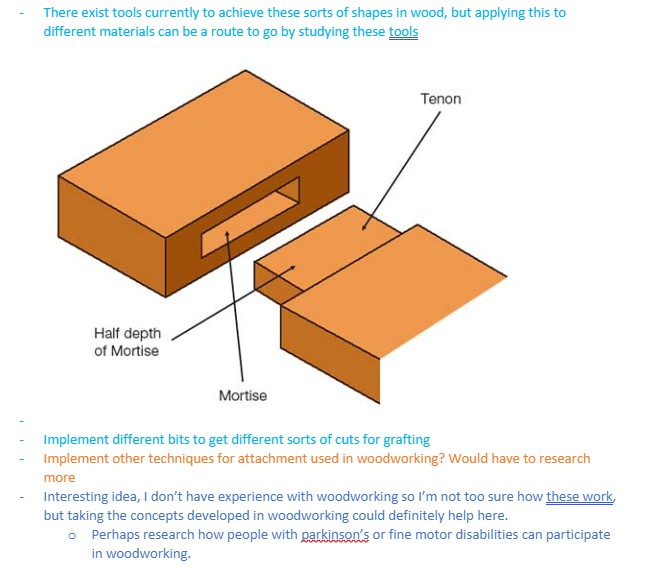
\includegraphics[width=\linewidth]{handbook/brainwriting.jpg}
    \end{column}
\end{columns}
\newpage
\begin{takeaway}
    Brainwriting is helpful when we want to go in more detail, and ensure that everyone's ideas come through.
\end{takeaway}
One helpful tip at later stages (i.e. re-divergence after some convergence) is to break up the opportunity into different aspects. Each person is responsible for coming up with initial ideas for each aspect and brainwriting is then performed.
\vspace{2mm}

I will refer to this as \textbf{segmented brainwriting}, and it should only be used once the group has agreed to go in a certain direction, or else there is a high risk of \textit{anchoring}.
}


\subsubsection{Biomimicry}
\frame[allowframebreaks]{\frametitle{Biomimicry}
\textit{Motivation:} Nature is the patient engineer, with certain traits optimized through millions of years of iterative natural selection. If possible, we should always look to the natural world to draw inspiration.
\begin{method}
    To perform biomimicry:
    \begin{enumerate}
        \item Identify the key elements of the opportunity
        \begin{itemize}
            \item This should be as generalized as possible to get more results, or else you risk being too specific
        \end{itemize}
        \item Perform research to see if nature replicates anything similar.
        \item With the new information, tighten the \textit{search space} by making the research progressively more specific to the design requirements.
        \item Discuss how one could mimic the properties / abilities extracted from the above process.
    \end{enumerate}
\end{method}
\newpage
\begin{example}
    In our Praxis I convergence sprint, our team looked at natural plant pots that existed in nature. Some examples included:
    \begin{itemize}
        \item Mushrooms growing on other plants
        \begin{itemize}
            \item Lead to a mushroom-cultivation device
        \end{itemize}
        \item Various natural mechanisms that slowly diffuse water / nutrients (i.e. other plants growing out of a host tree)
        \begin{itemize}
            \item Lead to diffusion mechanisms in an automated pot design
        \end{itemize}
    \end{itemize}
    \begin{center}
        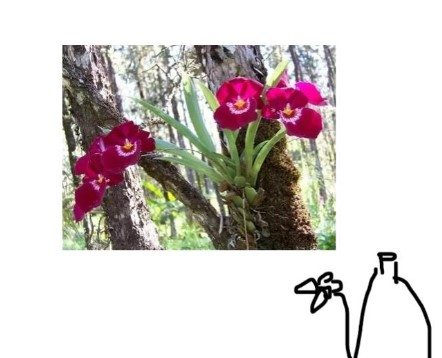
\includegraphics[width=0.35\linewidth]{handbook/biomimicry.jpg}
    \end{center}
\end{example}
}

\subsection{Reframing}
\frame[allowframebreaks]{\frametitle{Reframing}
% \begin{idea}
%     The \textbf{search space} is a term I borrowed from computer science. It represents the various types of solutions we consider during diverging (i.e. mechanical, electrical, large, small). We wish to maximize this domain during diverging.
% \end{idea}
\textit{Motivation:} It is very unlikely that the framing process was done perfectly. In fact, it doesn't need to. A good divergence would reveal flaws in the initial framing such as having:
\begin{itemize}
    \item too broad or narrow of a scope
    \item hidden assumptions that were not initially addressed
\end{itemize}
If there is a need, it is strongly recommended to go revisit framing.
\begin{example}
    When preparing for our Praxis II showcase, we initially tried to address all the parts of rose grafting. However, it became clear once we were brainstorming ideas that this was not feasible and we had to narrow our scope. 
\end{example}
}

\section{Converging}
\frame[allowframebreaks]{\frametitle{Converging}
The convergence process can be split into three sections:
\begin{itemize}
    \item Prototyping: Building and creating prototypes from initial design ideas
    \item Testing: Validating that the prototypes meet the criteria
    \item Iterating: Using holistic observations from the prototypes and the test results to eliminate, modify, and create new designs.
\end{itemize}
These don't have a specific order, rather it is very common for all three to occur simultaneously.
}

\subsection{Prototyping}
\frame[allowframebreaks]{\frametitle{Prototyping}
Prototyping is the process in which the initial design concept can get transformed into something with a higher fidelity, but it doesn't need to be super high quality!
\begin{idea}
    You should only try to prototype the most \textit{unbelievable} aspect of the design.
\end{idea}
Prototypes can include technical drawings, and quick visualizations using household objects. However, I consider them to be more useful for \textit{representing}, and I will focus on the three main tools used for higher fidelity prototypes:
\begin{itemize}
    \item 3D Printing
    \item Programming
    \item Mathematical
\end{itemize}
}

\subsubsection{3D Printing}
\frame[allowframebreaks]{\frametitle{3D Printing}
    \textit{Motivation:} Computer 3D models can be cool to look at, but are not practical if we want to conduct tests. 3D printing bridges this gap by easily printing almost any 3D model with little extra work:
    \begin{columns}
        \begin{column}{0.6\textwidth}
            \begin{example}
                I found it very hard to visualize one of my teammate's earliest ideas for Praxis II and if it was feasible. However, I was quickly able to 3D print it out and even conduct tests in a matter of hours. 
            \end{example}
        \end{column}
        \begin{column}{0.4\textwidth}
            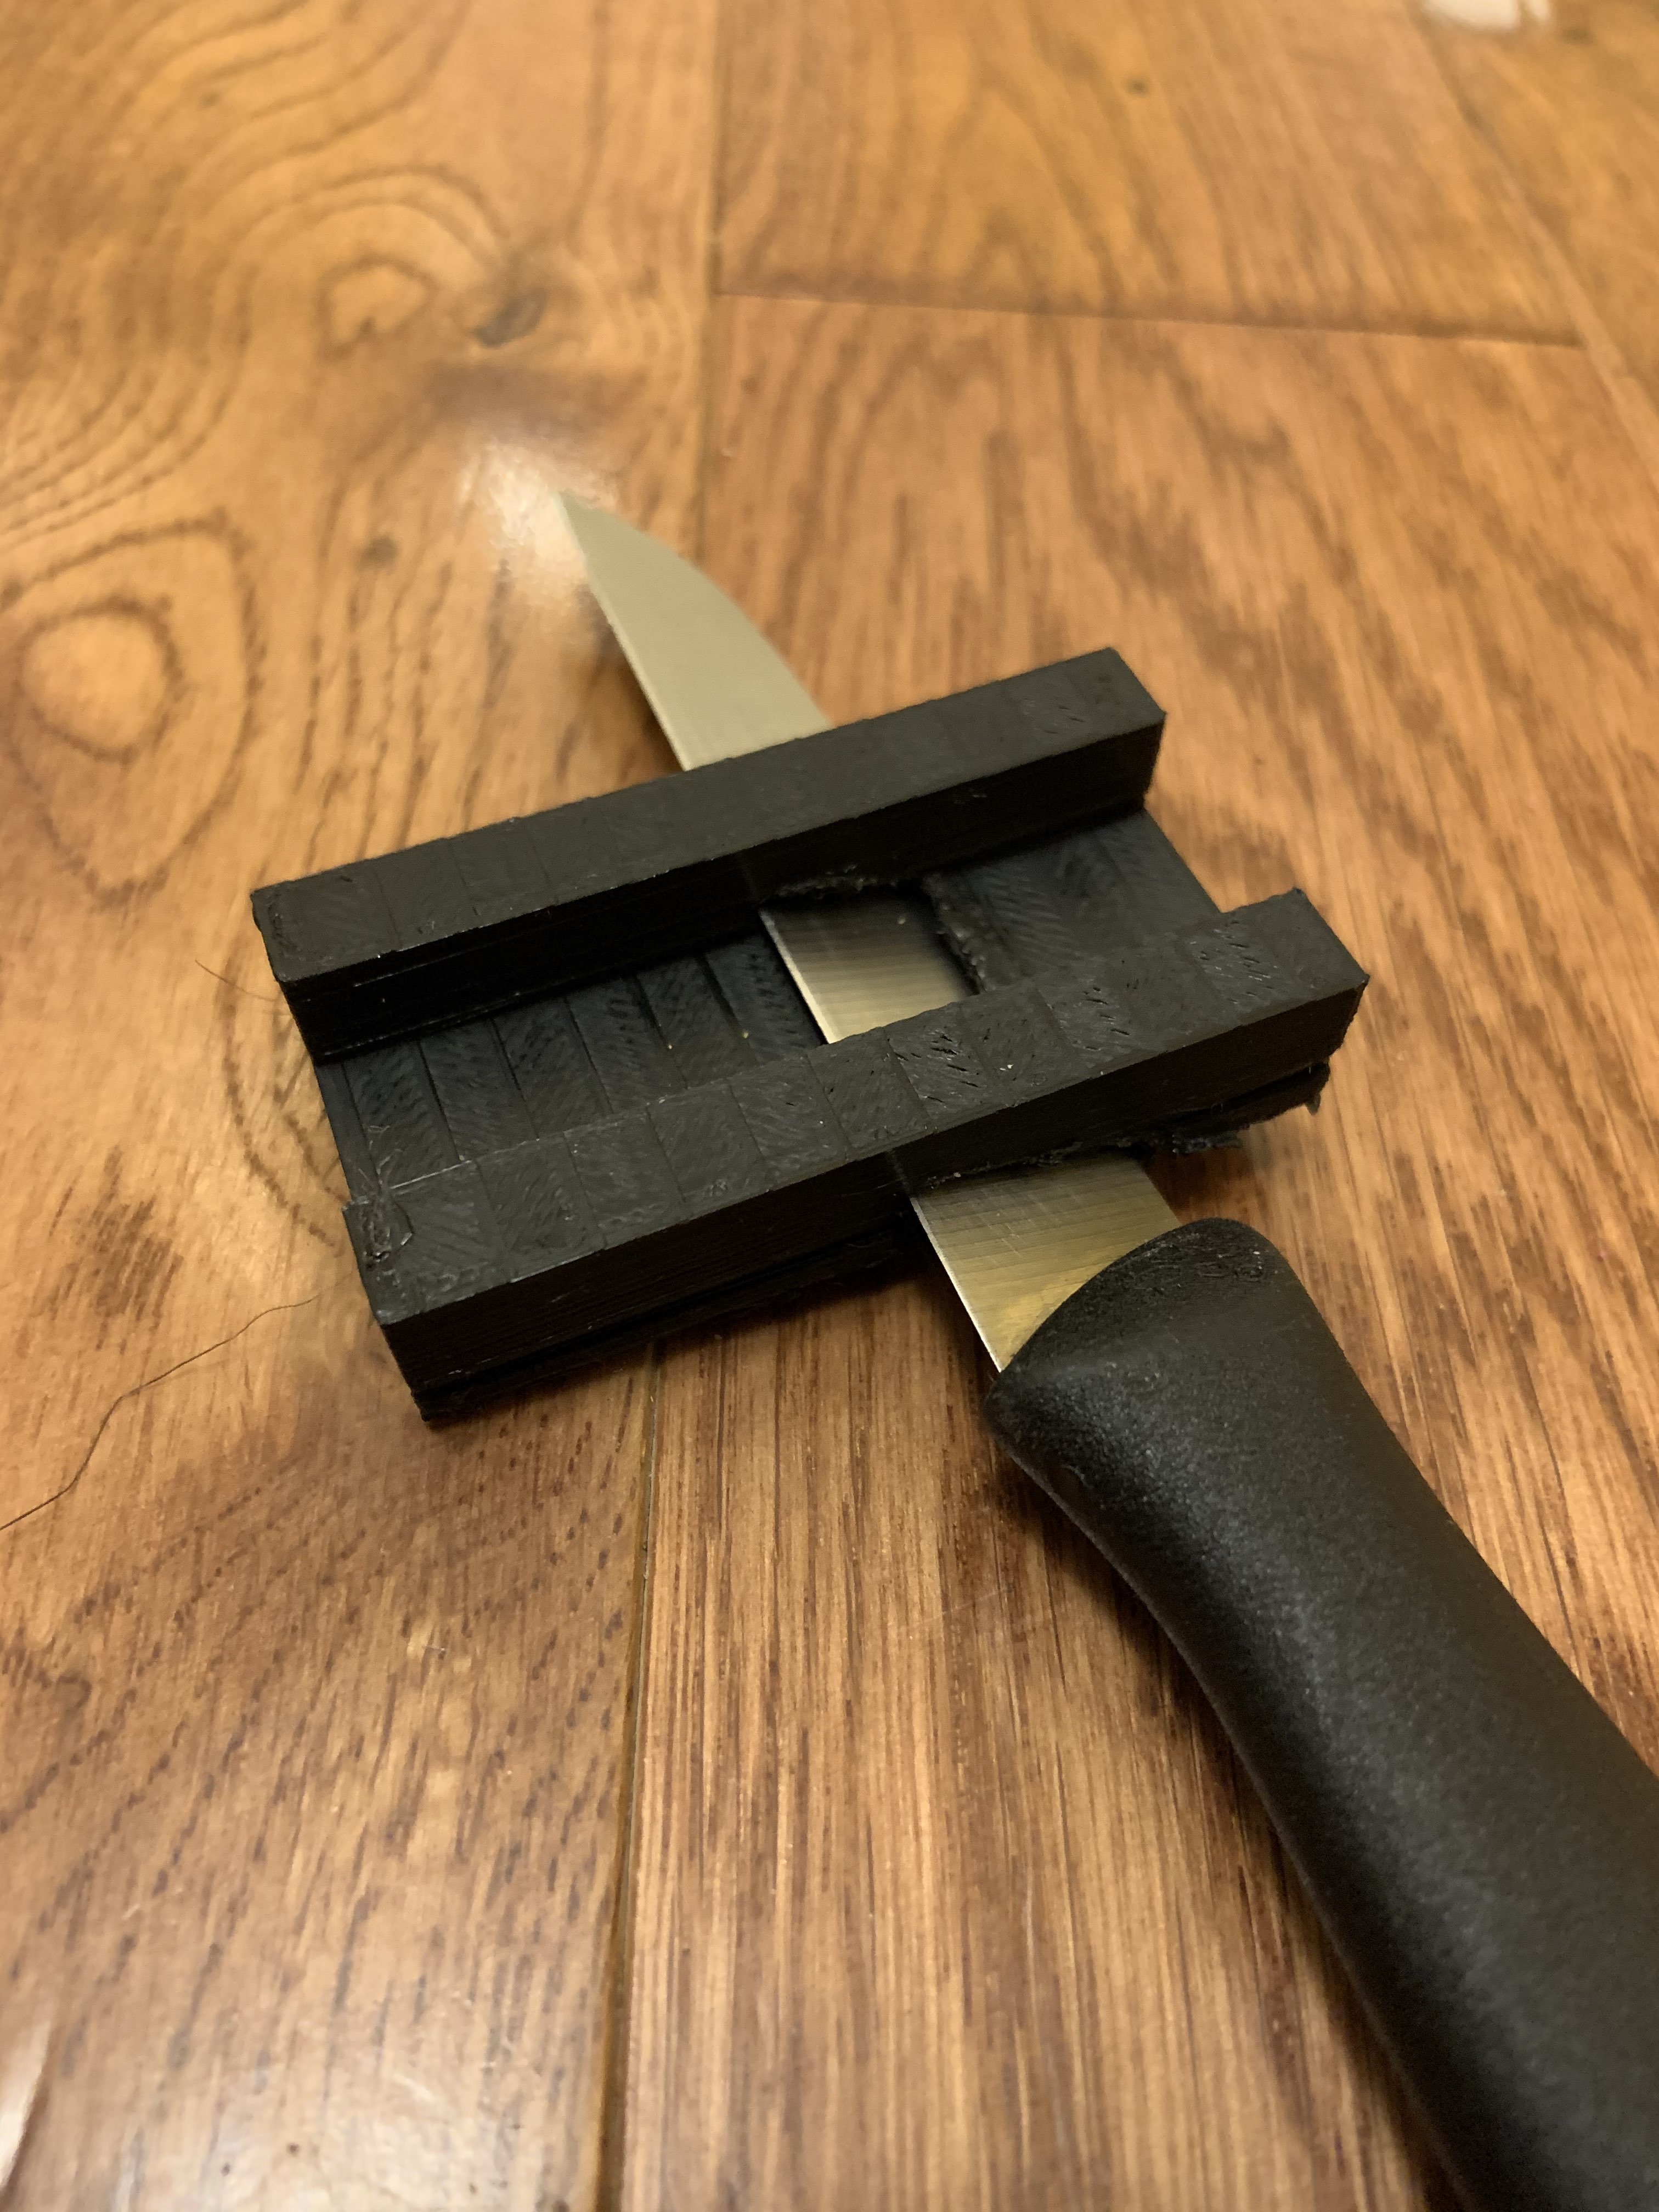
\includegraphics[width=\linewidth]{handbook/3d_printing.jpg}
        \end{column}
    \end{columns}
}

\subsubsection{Programming}
\frame[allowframebreaks]{\frametitle{Programming}
    \textit{Motivation:} If the design involves a digital component, it may be helpful to create a quick digital simulation of what the most critical part might look like. This can be done by searching related terms in the \textit{Github} search bar.
    \begin{example}
        For our Praxis I converging sprint, an idea was to use one's hand to control the computer (i.e. mouse free). A quick search on Github revealed over a thousand existing \textit{open source} projects.
        \begin{center}
            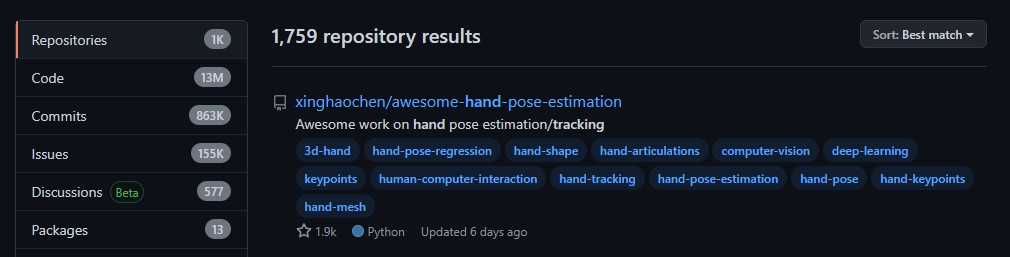
\includegraphics[width=0.8\linewidth]{handbook/github.jpg}
        \end{center}
    \end{example}

        I found the \textit{handtrack.js} library on Github and was able to use it to create a quick demonstration of using one's hand to control a cursor.
        \begin{center}
            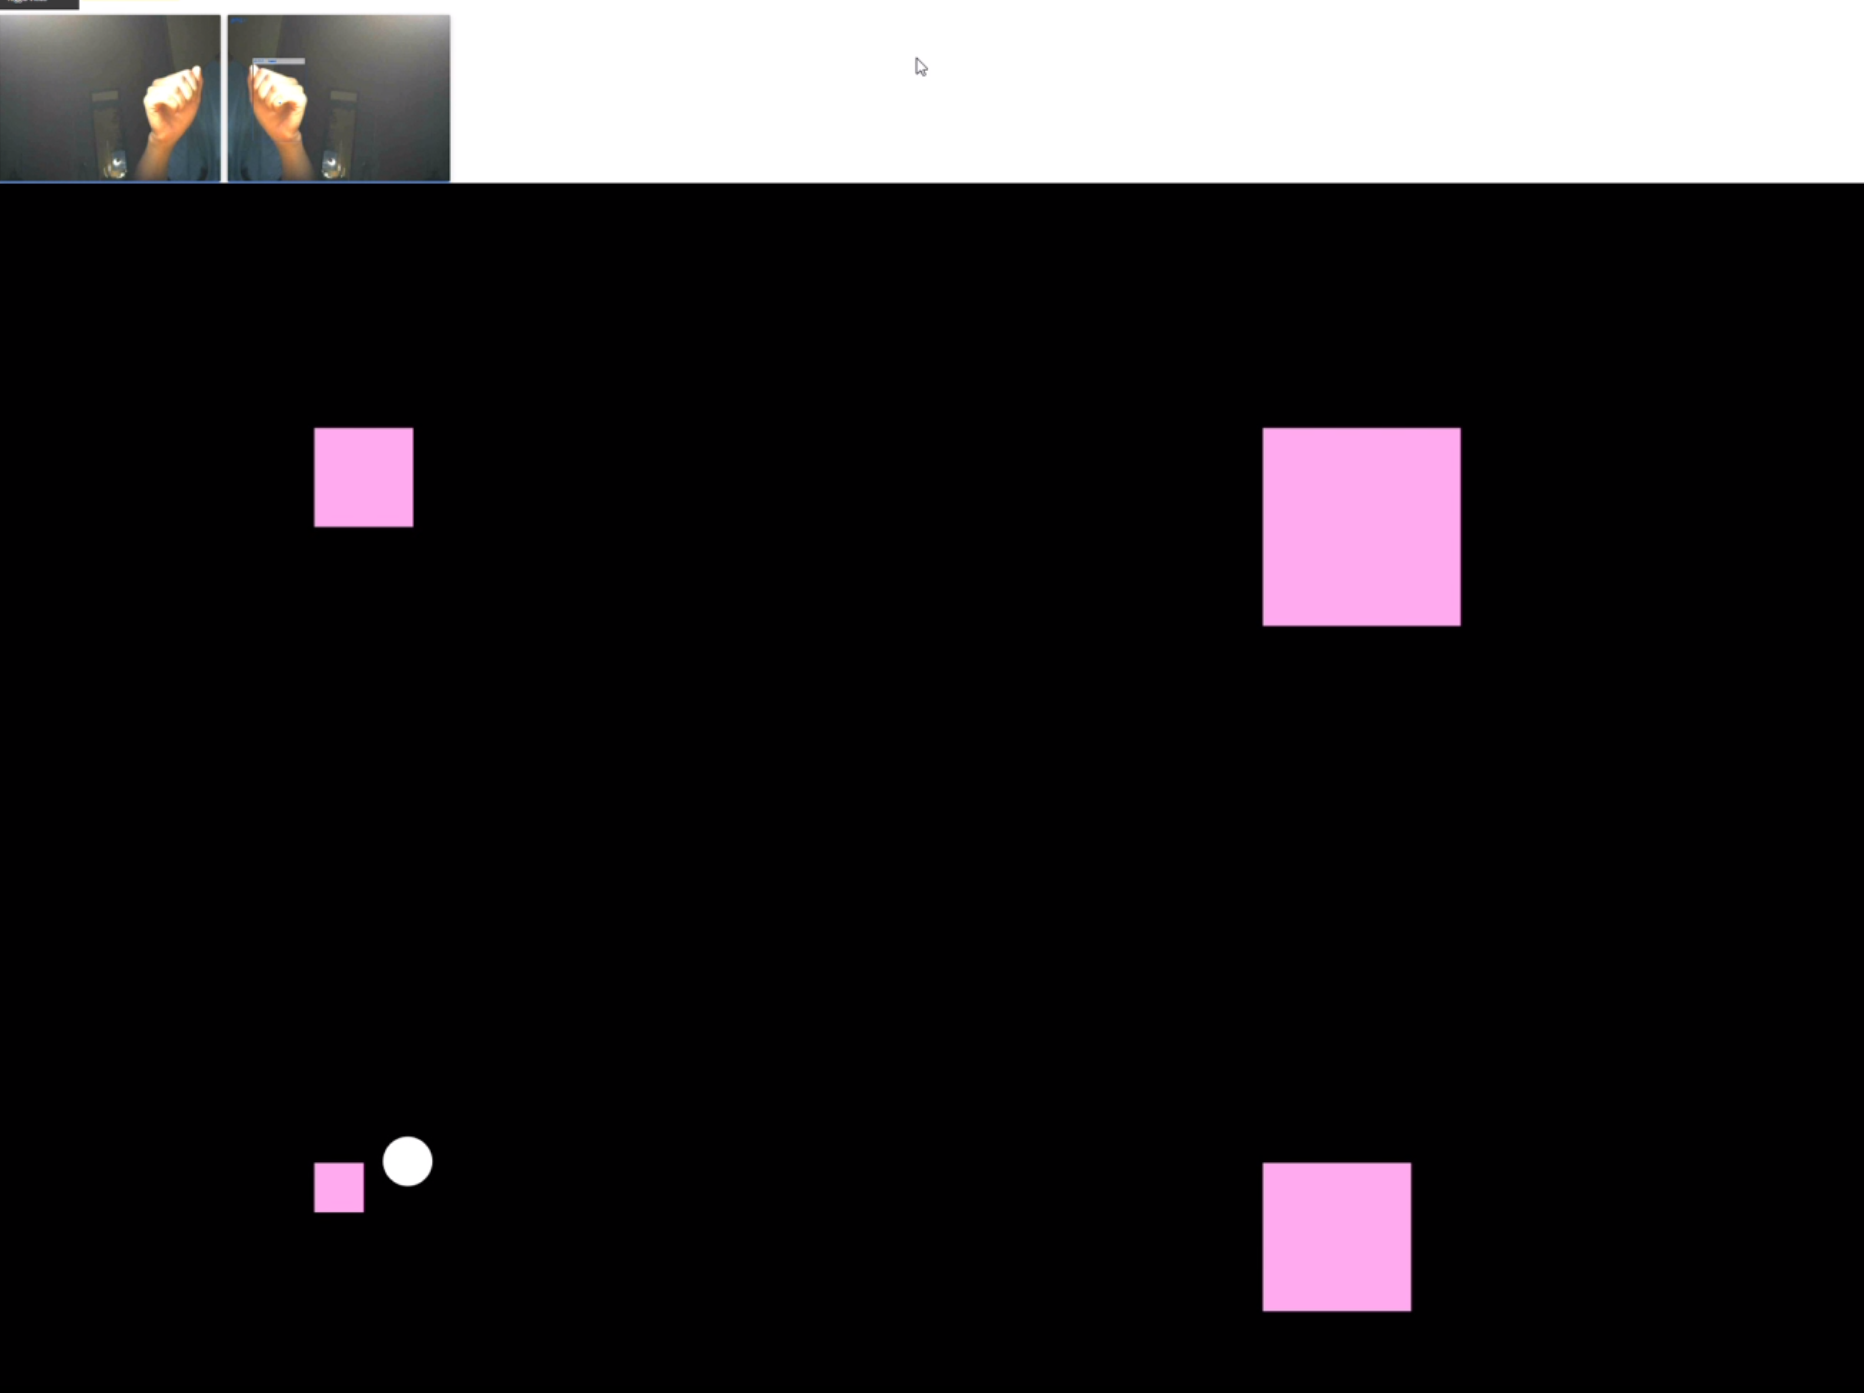
\includegraphics[width=0.5\linewidth]{handbook/handtrack.png}
        \end{center}
}

\subsubsection{Mathematical}
\frame[allowframebreaks]{\frametitle{Mathematical}
    \textit{Motivation:} For more complex designs, sometimes a mathematical model is sufficient to gauge the feasibility of a concept. We don't want to waste resources on something that isn't feasible.
    \begin{example}
        In our initial stages leading up to our Praxis II Beta release, one idea involved using gyroscopes to stabilize tools. I created a simple model of the gyroscope and used it to estimate the minimum rotational speed it must have to create noticeable effects.
        \begin{center}
            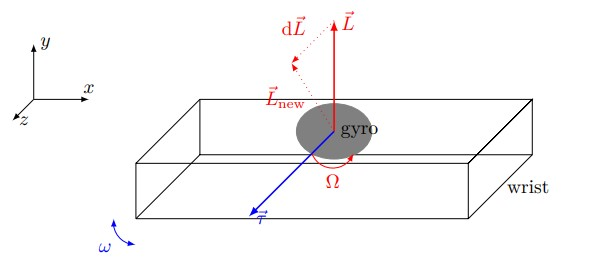
\includegraphics[width=0.5\linewidth]{handbook/gyroscope.jpg}
        \end{center}
        The number ended up to be $12,000\text{ rpm}$, and my team was not comfortable working with that fast a speed.
    \end{example}
}

\subsection{Testing}
\frame[allowframebreaks]{\frametitle{Testing}
    During testing, we wish to evaluate each design concept against the various metrics, and to ensure that they meet the constraints. However, there are several challenges:
    \begin{itemize}
        \item One may not always have access to the proper resources and technology to perform testing.
        \item It is easy to subconsciously bias the results towards one's initial assumptions if the test is not rigorous.
    \end{itemize}
    which I will attempt to address using two tools and frameworks: \textbf{designing proxies}, and the \textbf{bias factor correction}.
}

\subsubsection{Designing Proxies}
\frame[allowframebreaks]{\frametitle{Designing Proxies}
    \textit{Motivation:} As an engineering student, we won't always have access to the same resources professional engineers may use when performing industry standard tests. Sometimes, the test may require a final product from being completed. As a result, we need to find \textit{alternative} ways to test.
    \begin{example}
        Due to the covid-19 pandemic, our group did not contact anyone with Parkinson's to try our product: That would be unsafe and irresponsible. Our group also did not have Parkinson's, so it was a challenge making the claim that our tool can be used by someone with a tremor when none of us have tremors.
    \end{example}
    \newpage
    As a result, we had to artificially induce a tremor in ourselves with the use of exercise bands, which act as a \textit{proxy} for Parkinson's tremor. To show that this to some degree resembles Parkinson's tremor, we collected data using an accelerometer and performed a fast fourier transform to show the peak frequencies are in the right range.
    \begin{center}
        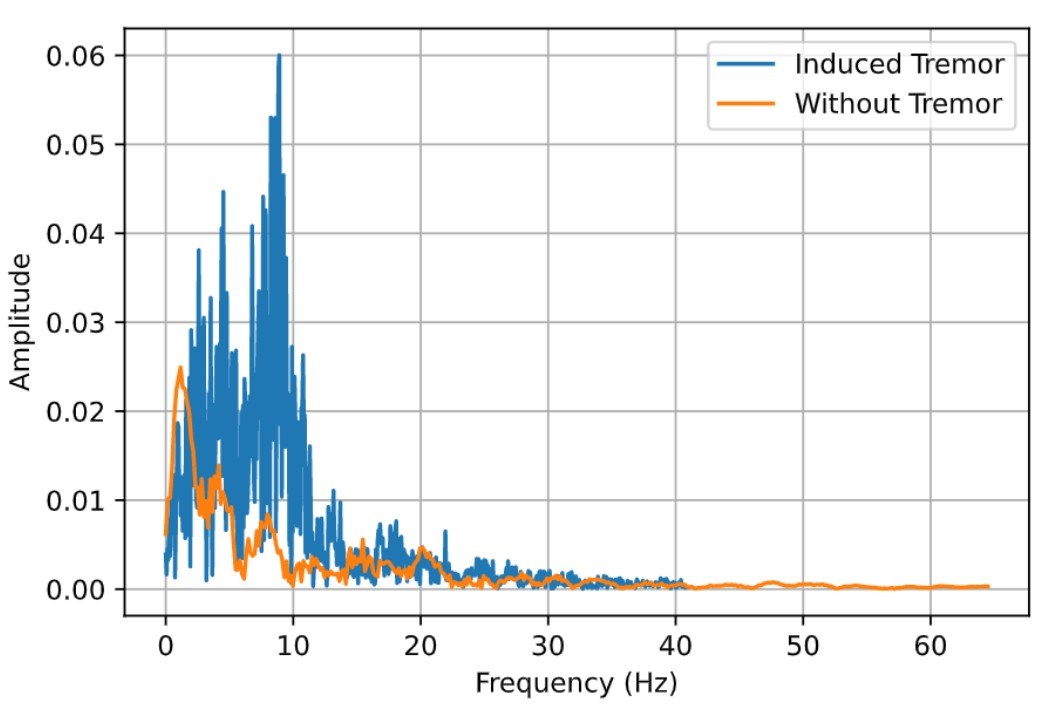
\includegraphics[width=0.65\linewidth]{handbook/fft.jpg}
    \end{center}
}

\subsubsection{Bias Factor Correction}
\frame[allowframebreaks]{\frametitle{Bias Factor Correction}
\textit{Motivation:} When a test is done by multiple people, then it is subject to bias and inconsistencies. During the converging sprint of Praxis I, my group invented a tool which I will call the \textbf{bias factor correction} (bfc) that attempts to mitigate this.
\begin{method}
    If there are $n$ people
    \begin{enumerate}
        \item Everyone performs a \textit{control} test (which should be similar to the final test) several times and records their individual average $a_i$.
        \item The total average is recorded as $\bar{a}$ and the correction factor $\text{bfc}_i$ for each person is:
        \begin{equation}
            \text{bfc}_i = \frac{\bar{a}}{a_i}
        \end{equation} 
        \item The final test is conducted, but the results each person should report is scaled by a factor of $\text{bfc}_i$.
    \end{enumerate}
\end{method}
\begin{example}
    In our Praxis I converging sprint, we conducted tests to see how long it took to navigate to a certain website using our different mouse designs. Since everyone used the mouse differently, it was crucial that we normalized our results with the BFC.
\end{example}
\begin{takeaway}
    One needs to be very careful justifying this technique when using it. Make sure the difference in results in the control is caused by minor differences and not huge misunderstandings of how to perform the test.
\end{takeaway}
}

\subsection{Iterating}
\frame[allowframebreaks]{\frametitle{Iterating}
Iteration is the process of narrowing down the set of ideas, and using those ideas to re-diverge. It consists of\cite{tools}:
\begin{itemize}
    \item \textbf{Multivoting:} A popular vote, used to decide which design choices should move forward.
    \item \textbf{Idea Advocate:} A debate style format where two teams are created, one advocating for a design, and one advocating against it.
    \item \textbf{Pugh Chart:} A more rigorous approach, comparing the designs against a reference.
    \item \textbf{SCAMPER:} An acronym designed to help incorporate different elements of different designs together to re-diverge.
\end{itemize}
\newpage
\begin{example}
    When I was creating the Gomoku AI, I did not explicitly use any of the converging tools I will discuss in the following slides, but I had a high level iteration process:
    \begin{enumerate}
        \item I first started with the most basic algorithm: mini-max
        \item I played games against the AI and had the AI play games against itself, and identified weaknesses.
        \item I did research on how to fix these weaknesses, and repeat.
    \end{enumerate}
    \begin{columns}
        \begin{column}{0.5\textwidth}
            An example game of Gomoku played between two AIs. In the next few slides, I will provide a rigorous process of performing iteration.
        \end{column}
        \begin{column}{0.5\textwidth}
            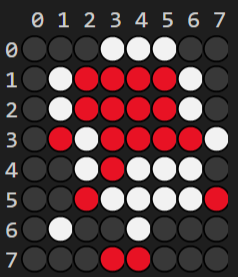
\includegraphics[width=\linewidth]{handbook/gomoku.png}
        \end{column}
    \end{columns}

\end{example}
}

\subsubsection{Multivoting}
\frame[allowframebreaks]{\frametitle{Multivoting}
\textit{Motivation:} At the start of the convergence phase, there could be several ideas which look very daunting. We don't know enough about each to make a rigorous judgement of what we should proceed with first, so we can cast a popular vote.
\begin{method}
    If there are $k$ ideas and $n$ people:
    \begin{itemize}
        \item Each person get around $\lfloor k/n \rfloor$ votes.
        \item Each person casts a vote for their top design choices. If they particularly like a design, they can cast more than one vote (though don't cast more than two, so that there's more variety)
        \item The votes are cast on an individual private document (to prevent bias), and after everyone is done, recorded on a public sheet.
        \item Around the top $n$ ideas are pursued.
    \end{itemize}
\end{method}
\begin{example}
    My teams used this to decide which prototypes we should build first in both our Praxis I converging sprint an for Praxis II showcase.
    \begin{center}
        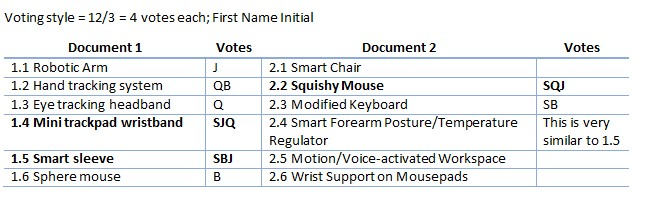
\includegraphics[width=0.8\linewidth]{handbook/multivoting.jpg}
    \end{center}
\end{example}
\begin{takeaway}
    This method is the least rigorous and should only be used when the initial set of ideas is really large. Do \textit{not} ignore the ideas that were not chosen. You can always come back to those later.
\end{takeaway}
}

\subsubsection{Idea Advocate}
\frame[allowframebreaks]{\frametitle{Idea Advocate}
\textit{Motivation:} Team members can sometimes be \textit{too} nice. The general philosophy during divergence is to be as open minded as possible and not critique and this mindset often carries over to converging, where it is necessary to examine each design critically.
\begin{method}
    If a team consists of $n$ people,
    \begin{enumerate}
        \item Make two roughly even teams for each idea. For diversity, try to ensure that the teams are different for each idea (i.e. There are roughly $\frac{1}{2}\binom{n}{2}$ ways of picking a unique team.)
        \item Each side gets a fixed amount of time to present their case, and free debate can occur for a fixed amount of time. Notes should be taken.
        \item Switch to the next design idea.
    \end{enumerate}
\end{method}
\newpage
\begin{example}
    After some re-divergence in Praxis II showcase, we performed the idea advocate activity. A screenshot is shown below. Notice the names indicating who is on which team and the notes we took during the debate:
    \begin{center}
        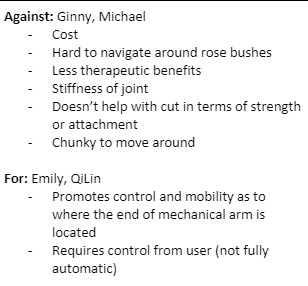
\includegraphics[width=0.45\linewidth]{handbook/idea_advocate.jpg}
    \end{center}
\end{example}
However, this isn't perfect. We often found that we were making arguments that were not backed up. For example, the argument that the device was \textit{hard to navigate around rose bushes} was generated from intuition, as we had to come up with the arguments on the spot.
\begin{takeaway}
    It is probably a good idea to plan out the arguments before meeting with the group so they can be more thought out. This will involve assigning teams the previous meeting. 
\end{takeaway}
This is a great way of getting a better holistic understanding of the different designs. \textbf{Multivoting} could be performed afterwords if the sample size is still too big.
}

\subsubsection{Pugh Chart}
\frame[allowframebreaks]{\frametitle{Pugh Chart}
\textit{Motivation:} We need a rigorous way of determining the best designs using the results from testing.
\begin{method}
    \begin{enumerate}
        \item Select a reference design. This could be an existing solution or a design that you holistically feel is in the middle (better than some, worse than some). This can always be changed later.
        \item Create a table with designs and metrics, with metrics sorted from most to least important.
        \item Using the criteria for each metric, write down if each design did better or worse than the reference for a specific criteria.
        \item Use the final table to make a final judgement. 
    \end{enumerate}
\end{method}
\newpage
\begin{example}
    This is the pugh chart we made for our Praxis I converging sprint:
    \begin{center}
        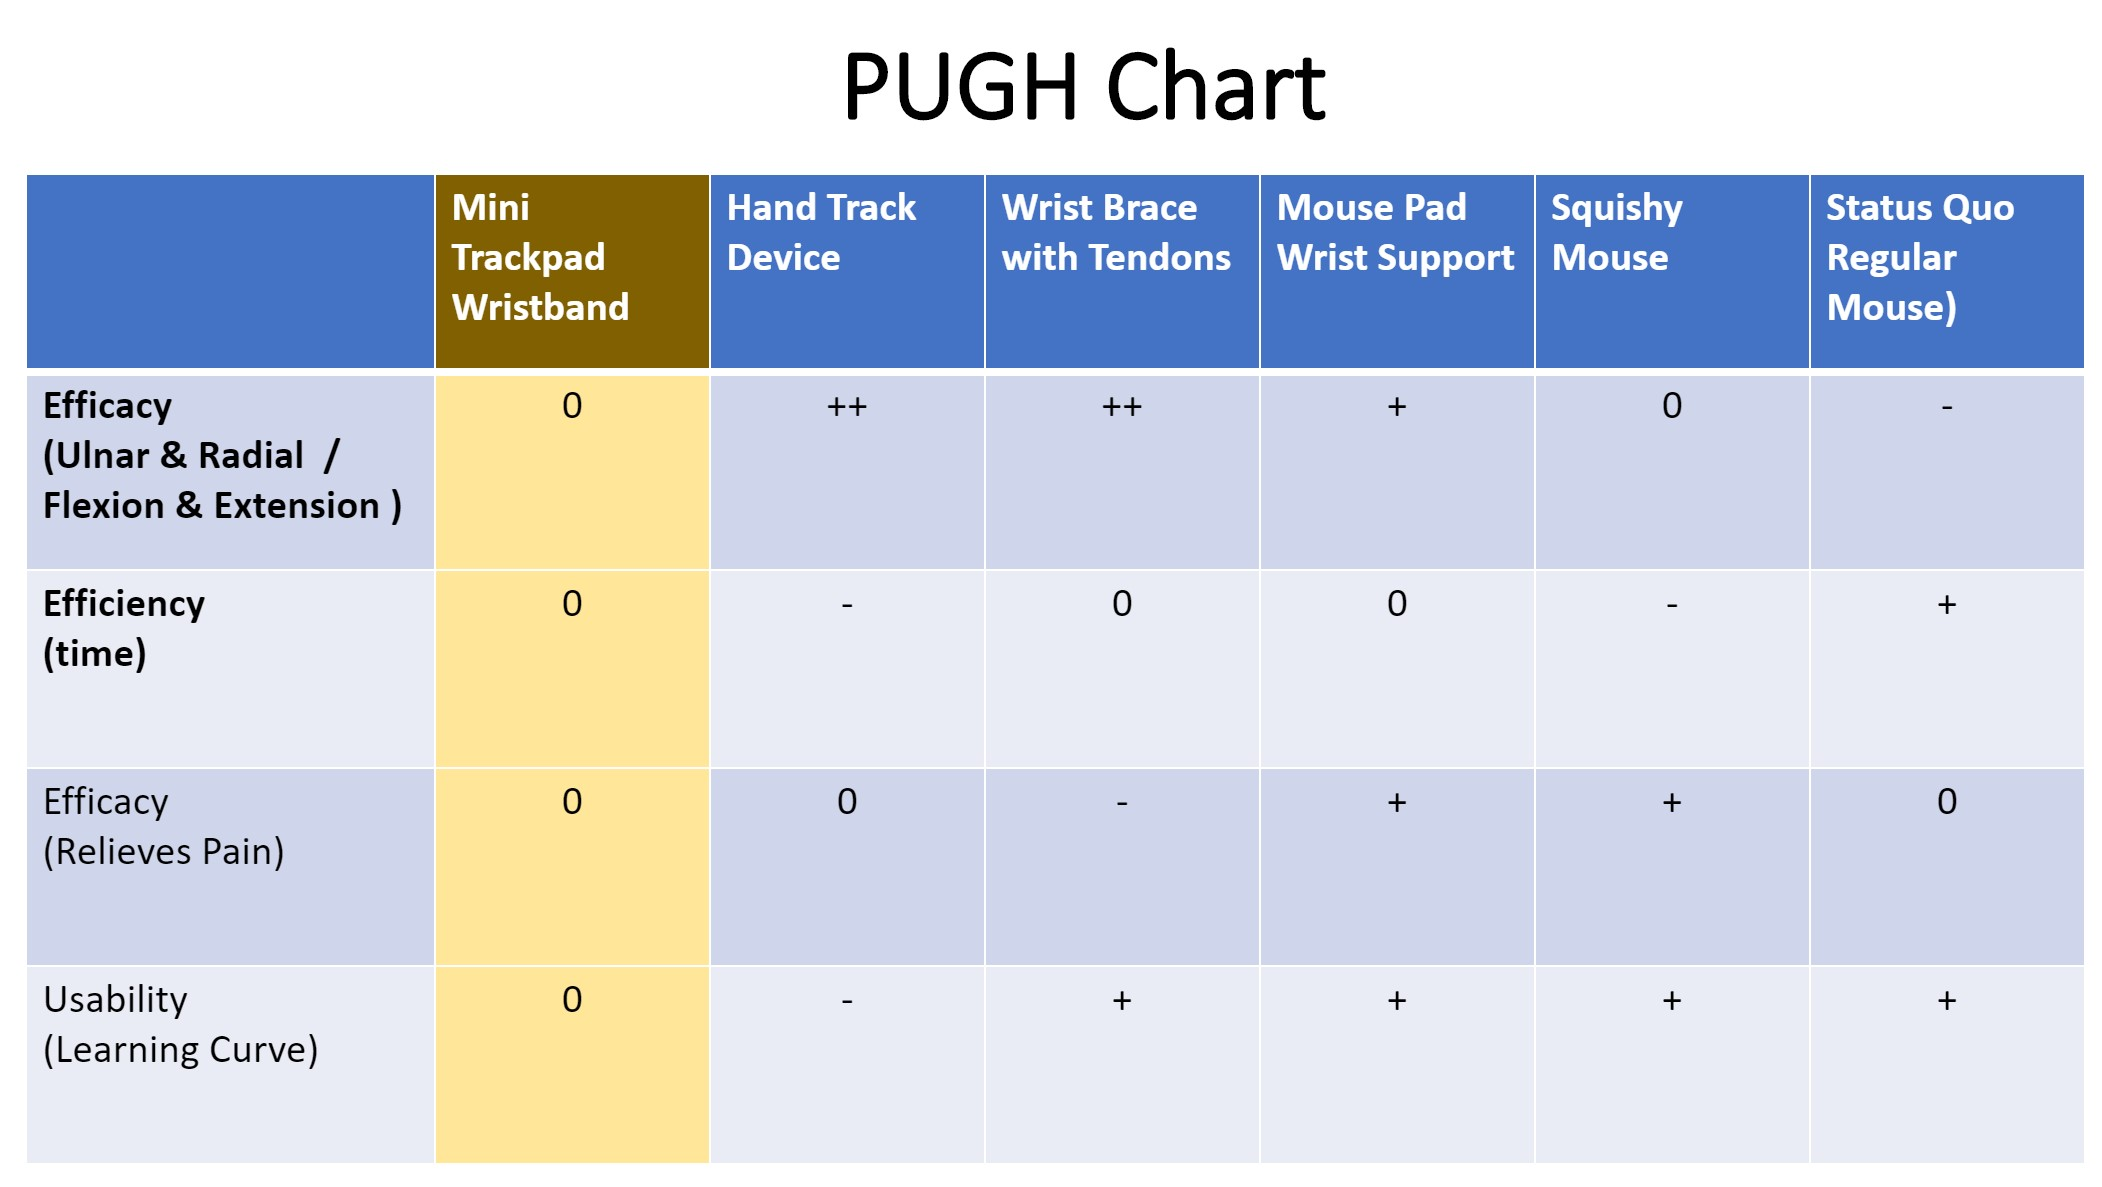
\includegraphics[width=0.85\linewidth]{handbook/pugh.jpg}
    \end{center}
\end{example}
Notice we introduced $++$ to signify that it performed extremely well against a certain criteria.
\newpage

Using this chart, we made the claim that the mouse pad wrist support was the best option. Even though it didn't outperform the hand track and wrist brace devices in every component, it did not perform worse than our reference.
\begin{warning}
    Do \textit{not} assign numbers to each cell and add everything up. The final decision should be a \textit{well justified} holistic decision. Do not \textbf{hide behind numbers.}
\end{warning}
\begin{takeaway}
    It may also be a good idea to supplement a Pugh chart with a \textbf{measurement matrix}, where the column and row headers stay the same, but the actual test results are inputted. This gives other people a way to judge for themselves the difference between ``performs much better'' and ``performs better.'' For example, we made the following matrix when picking the best bridge during our CIV project:
    \begin{center}
        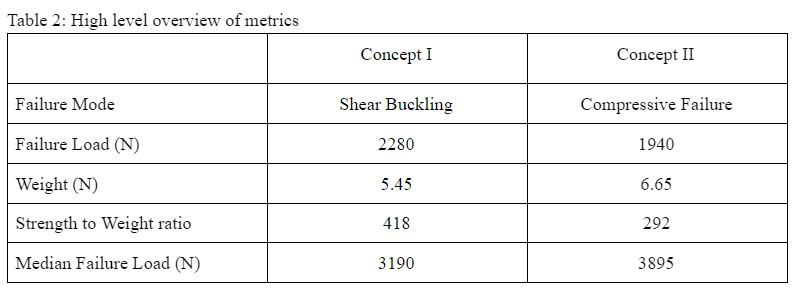
\includegraphics[width=0.9\linewidth]{handbook/measurement matrix.jpg}
    \end{center}
\end{takeaway}
}

\subsubsection{SCAMPER}
\frame[allowframebreaks]{\frametitle{SCAMPER}
\textit{Motivation:} It is unlikely that one of the initial ideas generated will be the final design. It is often a good idea to look at the candidates and use them as inspiration to generate more ideas.
\begin{method}
    SCAMPER is an acronym for \textbf{Substitute}, \textbf{Combine}, \textbf{Adapt}, \textbf{modify}, \textbf{put to another use}, \textbf{eliminate}, and \textbf{reverse}.
\end{method}
We can ask the following guiding questions for each element in SCAMPER:
    \begin{itemize}
        \item \textbf{Substitute}: Could some part of the design be substituted by something else?
        \item \textbf{Combine}: Could we combine two or more other ideas together?
        \item \textbf{Adapt}: Could we take an existing design and adapt it to this design?
        \item \textbf{Modify}: Could we modify part of the opportunity (i.e. reframing)? Would the design work differently if that happened? 
        \item \textbf{Put to another use}: Could we take an element in this design and put it to another use somewhere else?
        \item \textbf{Eliminate}: Are there any parts of our design that are redundant that we can eliminate?
        \item \textbf{Reverse}: What if we reversed the purpose of the design (i.e. made it so that it fails constraints). Can we learn anything from that?
    \end{itemize} 
    \newpage
    \begin{example}
        Leading up to our Praxis II showcase, we applied SCAMPER after we have created concept sketches and discussed each of our top design ideas:
        \begin{center}
            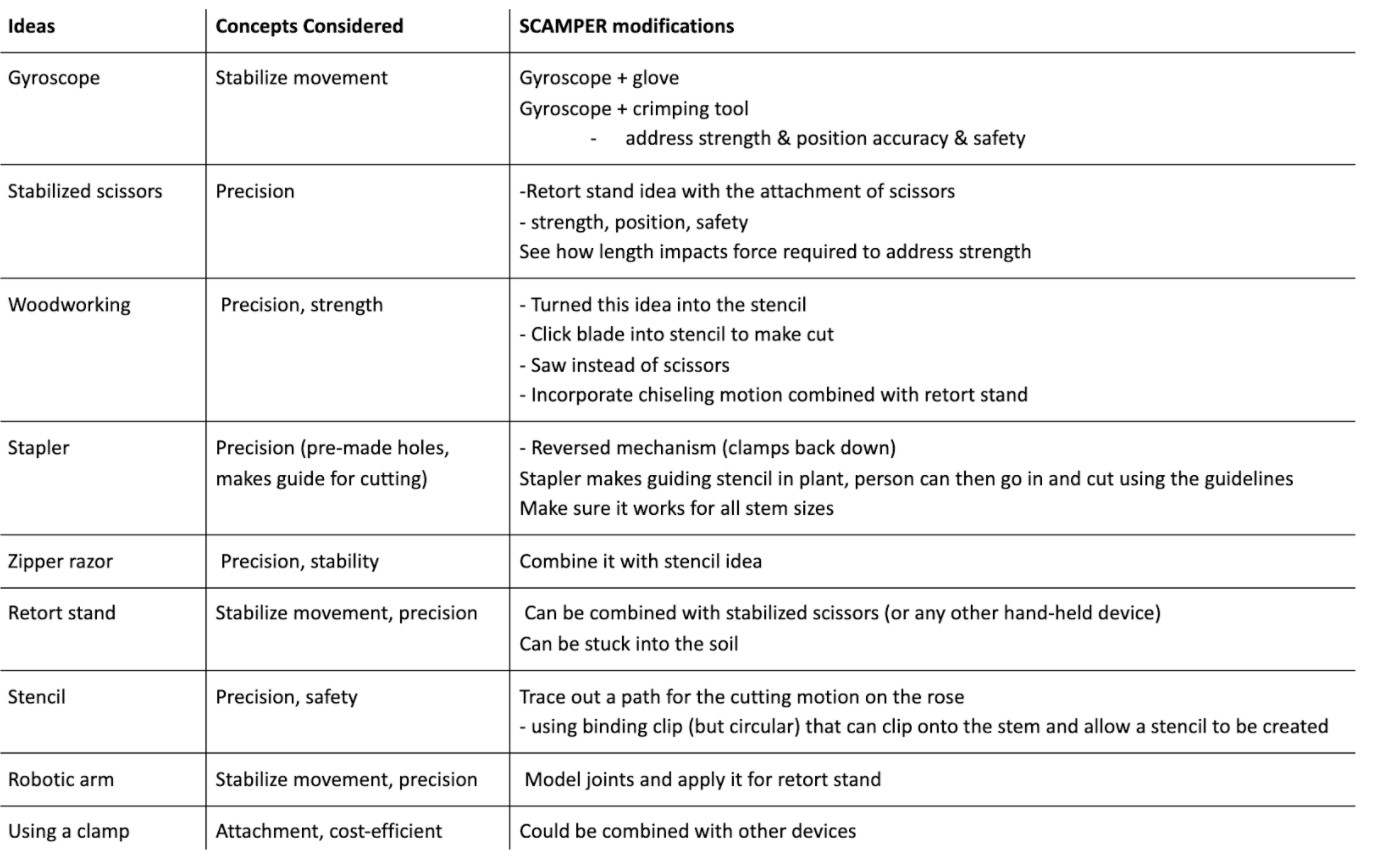
\includegraphics[width=0.8\linewidth]{handbook/scamper.jpg}
        \end{center}
    \end{example}
    One problem we experienced was that due to the large amount of ideas, we were only able to do part of SCAMPER for each. The notes we took were very brief, and we didn't carefully think through all the components.
    \begin{takeaway}
        SCAMPER should only be used once the set of candidate ideas is more narrow. This allows for a more comprehensive re-diverging by considering the problem at all possible angles.
    \end{takeaway}
}
\section{Presenting}
\frame[allowframebreaks]{\frametitle{Presenting}
Not only is it important to perform good engineering design, it is also important to communicate it effectively.
\vspace{2mm}

Creating good team dynamics has several important components. However, I will only focus on one specific element: communicating across design ideas.

}
\subsection{Prototyping}
\frame[allowframebreaks]{\frametitle{Prototyping}
\textit{Motivation:} In the \textit{diverging} section, I talked about \textit{prototyping for testing}. However, lower fidelity prototypes are also extremely important in order to eliminate pre-conceived assumptions and to ensure the entire team understands what you're thinking of. This can involve:
\begin{itemize}
    \item A quick drawing.
    \item Using household objects. Some of the most useful items I found were:
    \begin{itemize}
        \item Paper
        \item Tape
        \item Scissors
        \item Pencils
        \item Cardboard
    \end{itemize}
\end{itemize}
\newpage
\begin{example}
    For our Praxis II showcase, one of my colleagues suggested an idea using a ``hinge.'' No matter how many times he tried to explain it, I could not picture how it works. However, using some cardboard he was able to quickly prototype something:
    \begin{center}
        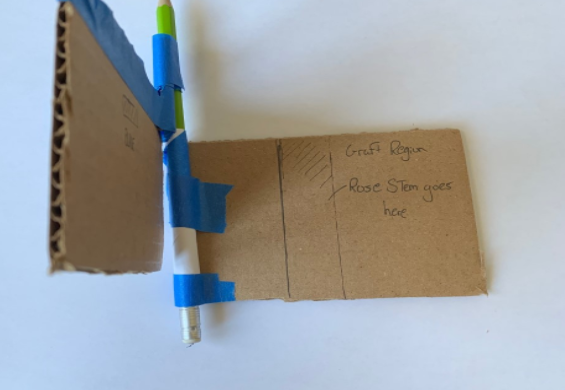
\includegraphics[width=0.5\linewidth]{handbook/hinge.png}
    \end{center}
    While it can't be used to cut roses, it gave me a better understanding of his idea.
\end{example}
}

\subsection{Works Cited}
\frame[allowframebreaks]{\frametitle{Works Cited}
\printbibliography
}
\end{document}
